\subsection{Hardware - V2.1}

    This version of the basic node had minor changes to the hardware. 

    \subsubsection{Serial Port}

        It lacked an laid out Serial Interface, which was added in V2.2.
        During the software development of the basic node, it happened that the 
        programming over the nativ USB of the ESP32 C3 was not possible. Duo to 
        setting buildflags, that would disable USB programming. To make programming
        easier and fix this issue, the serial interface laid out on the PCB. 


    \subsubsection{Module-Detection}
        While testing with this version, it was noticed that pin 3 was floating,
        potentially causing the base module to regonize a module without one being attached.
        To fix this issue in V2.2, the voltage divider on the modules were split up and
        a 100kOhm resistor was added to pull the pin to GND on the base module.
        
    \subsubsection{PCB - V2.1}
        The size of the PCB is identical to V2.2 with a footprint of 30x70mm. 

    \begin{figure}[H]
        \centering
        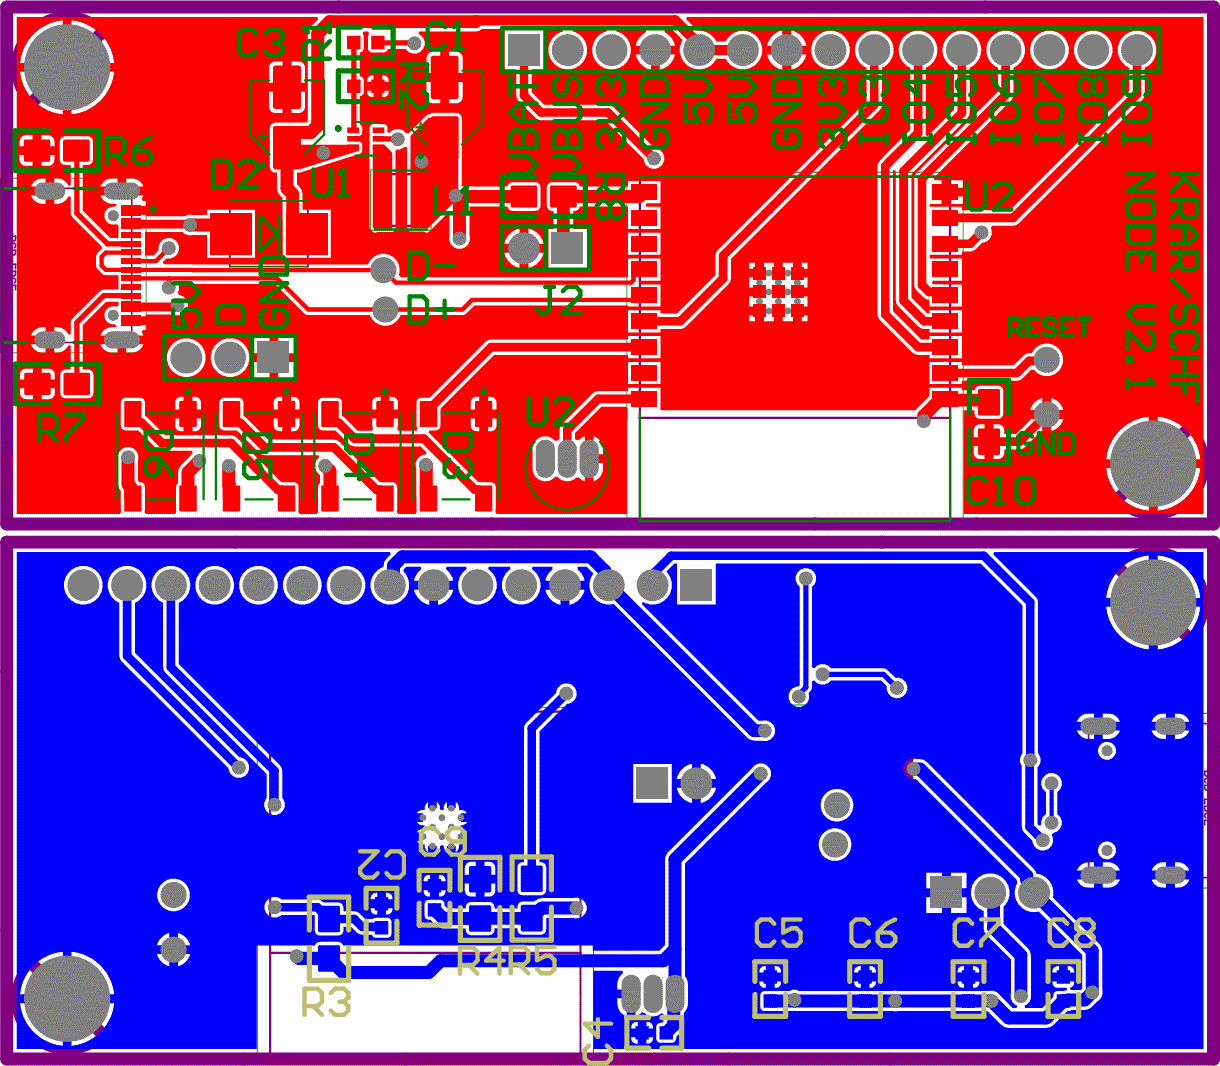
\includegraphics[width=1\textwidth]{assets/HW/PCB-NODE-V2.1.png}
        \caption{PCB of the basic node V2.1. [Red - Frontside, Blue - Backside]}
    \end{figure}


\subsection{Hardware - V2.0}

    This version of the basic node had major changes to the hardware. Following flaws
    were disscovered in V2.0:

    \subsubsection{Ground-Plane}
        The ground-plane was removed underneath the ESP32-C3 to improve the
        signal quality. 

    \subsubsection{Spare-Header}
        One GPIO of the MCU was not used, so it was decided to add a pinheader to the basic node.
        Where a button or magnetic switch could be attached to. When pressed or triggered, the
        button could be used to interact with the node or trigger a specific action.

    \subsubsection{PCB - V2.0}
        The size of the PCB is identical to V2.1 with a footprint of 30x70mm.
        
    \begin{figure}[H]
        \centering
        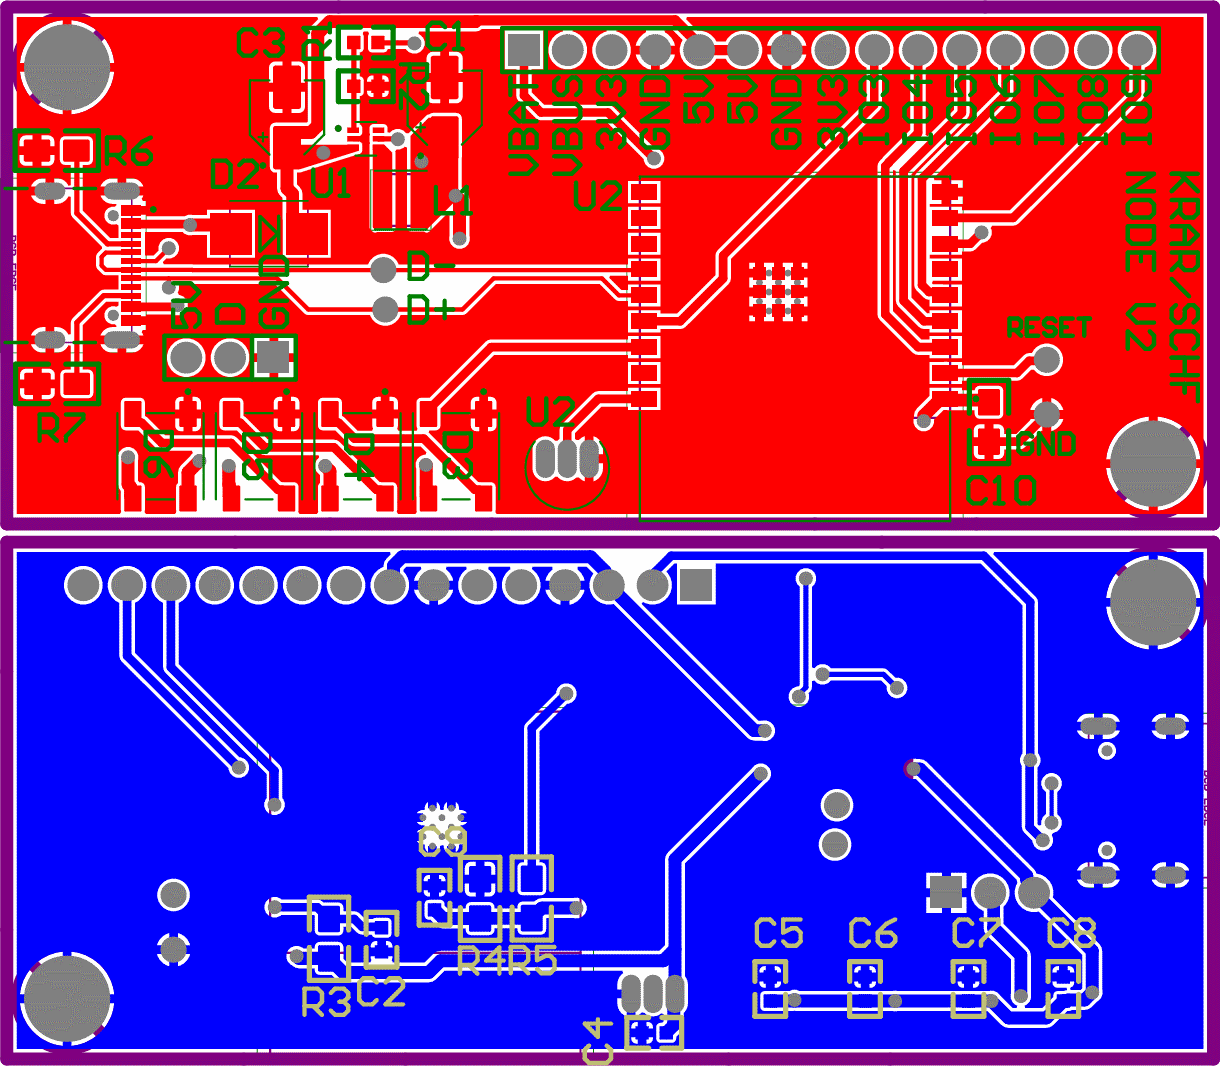
\includegraphics[width=1\textwidth]{assets/HW/PCB-NODE-V2.0.png}
        \caption{PCB of the basic node V2.0. [Red - Frontside, Blue - Backside]}
    \end{figure}
